
%(BEGIN_QUESTION)
% Copyright 2007, Tony R. Kuphaldt, released under the Creative Commons Attribution License (v 1.0)
% This means you may do almost anything with this work of mine, so long as you give me proper credit

In the study of basic electricity, we generally assume the travel speed of electrical signals to be infinite.  For example, we assume the LED will energize {\it immediately} when the transistor turns on in this circuit:

$$\includegraphics[width=15.5cm]{i02179x01.eps}$$

However, we know the effects of electricity cannot travel beyond a certain maximum speed: the speed of {\it light}.  Estimate the delay in time between the transistor's turning on and the LED's lighting up, assuming the cable connecting the two is 100 km (kilometers) in length.

\vskip 20pt \vbox{\hrule \hbox{\strut \vrule{} {\bf Suggestions for Socratic discussion} \vrule} \hrule}

\begin{itemize}
\item{} Suppose the characteristic impedance ($Z_0$) of the cable did not match the resistance of the LED and dropping resistor.  How long would it take the reflected signal to reach the source from the time the transistor turned on?
\item{} Real cables have {\it velocity factors} less than unity.  Explain how this realistic effect will impact your calculations of delay time for a real cable.
\item{} Explain how an E-type MOSFET is turned on and off, identifying the necessary gate-source voltage necessary to stimulate it into saturation and cutoff.
\end{itemize}

\underbar{file i02179}
%(END_QUESTION)





%(BEGIN_ANSWER)

Distance is equal to velocity multiplied by time:

$$x = vt \hskip 30pt t = {x \over v}$$

We know that the length of the cable in this circuit is 100 km (100 $\times$ 10$^3$ m).  Assuming a velocity factor of 1:

$$t = {100 \times 10^3 \hbox{ m} \over 3 \times 10^8 \hbox{ m/s}}$$

$$t = 333.3 \mu \hbox{s}$$

\vskip 10pt

Any reflected signals will take twice as long as this to travel down the cable and back.


%(END_ANSWER)





%(BEGIN_NOTES)


%INDEX% Electronics review: characteristic impedance of transmission line
%INDEX% Electronics review: surge impedance of transmission line

%(END_NOTES)


